
\section{IAD $\supseteq $ RDP $\times$ SMA }
%------------------------------------------------------------------------
\begin{frame}

\begin{center}
{\huge Capítulo 3 -- IAD $\supseteq $ RDP $\times$ SMA }
\end{center}

\end{frame}

%------------------------------------------------------------------------
\begin{frame} %[allowframebreaks=0.9]


\frametitle{O que vai ter neste capítulo}

\begin{itemize}
  \item Mais conceitos sobre SMA dentro da IAD ... vantagens etc
  \item Quando a RDP é mais interessante (e quando não é)
  \item Vantagens da SMA (e desvantagens com relação a RDP)
\end{itemize}


\end{frame}

%------------------------------------------------------------------------


\begin{frame} %[allowframebreaks=0.9]


\frametitle{Porque distribuir?}

\begin{itemize}
  \item Sistemas em geral são distribuídos \textbf{funcionalmente}
  \pause
  \begin{itemize}
    \item Devido uma especificação
    \item Devido uma especialização
    \item Dividir e diminuir a complexidade $\rightarrow$ decompor o problema
    
  \end{itemize}

  \pause
  \item Sistemas em geral são distribuídos \textbf{fisicamente}
  \pause  
  \item Finalmente, na \textbf{resolução de problemas} (em geral): 
  há alguns cuja solução é inerentemente distribuída ou 
  fica mais fácil distribuindo!
  

\end{itemize}


\end{frame}
%------------------------------------------------------------------------


\begin{frame}

  \frametitle{Motivando ao  distribuído}
        
\begin{figure}[!ht]
\centering
%\includegraphics{}
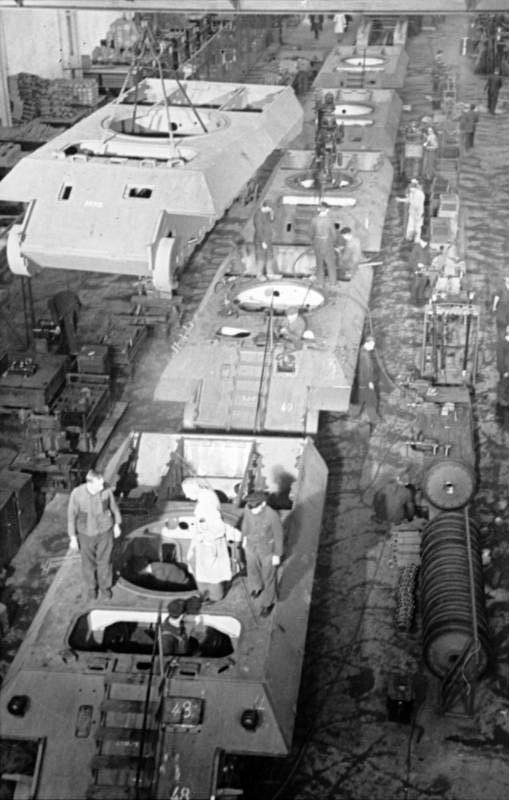
\includegraphics[height =.6\textheight,width=.4\textwidth]{figuras/fabrica_tanques.jpg}
\caption{Ações paralelas, distribuídas, concorrentes ... e tudo planejado!}
%\label{ag_01}
\end{figure}
    
   
\end{frame}


%------------------------------------------------------------------------


\begin{frame} %[allowframebreaks=0.9]


\frametitle{IA Distribuída}

\begin{itemize}
  \item Entidades (ou várias) que interagem sob uma:
  \begin{itemize}
    \item Organização (há uma conexão entre as partes)
     \item Ação 
     \item Interação
  \end{itemize}

     \item Metáfora usada de inteligência: \textcolor{blue}{\textbf{comportamento  social}} (sim, os dos seres animais, incluindo o \textit{homo-sapiens}!)
\end{itemize}


\end{frame}

%------------------------------------------------------------------------

\begin{frame} %[allowframebreaks=0.9]


\frametitle{Resumindo a IAD}

\begin{itemize}
    \item Não é IA paralela (esta é voltada em paralelizar computacionalmente as implementações em IA), nem Sistemas Distribuídos. 
  
    \item Um resolução grupal de problemas, através de  \textit{cooperação} (diferente de \textit{colaboração}).
    
    \item Grande interatividade e capacidade de comunicação.

     \item Organização - meios que garantam a \textit{convergência}: 
      estruturas de autoridade e controle divididos. 

     \item Divisão de conhecimento (nota: \textit{o que é conhecimento?}) e recursos
     
\end{itemize}


\end{frame}

%------------------------------------------------------------------------


\begin{frame} %[allowframebreaks=0.9]


\frametitle{IA Distribuída: 
dois tipos de sistemas}

\begin{itemize}

  \item Resolução Distribuída de Problemas (RDP)
  \begin{itemize}
    \item consciência do objetivo global e divisão clara de tarefas
     \item Exemplos: robótica clássica, busca na Web, gerência de sistemas distribuídos, ...
  \end{itemize}
 
 \item Sistemas Multiagentes (SMA)
    
     \begin{itemize}
       \item não consciência do objetivo global e nem divisão clara de tarefas
       \item Exemplos: n-puzzle, futebol de robôs, balanceamento de carga, robótica, ...

     \end{itemize}

     \end{itemize}
\end{frame}


%------------------------------------------------------------------------


\begin{frame} %[allowframebreaks=0.9]


\frametitle{Porque usar a metáfora de agentes?}

\begin{itemize}
  \item Fornece metodologias de desenvolvimento de sistemas  inteligentes estendendo as de engenharia de software
   \item Fornece visão unificadora das várias sub-áreas da IA 
  \item  Ajuda a embutir a IA em sistemas computacionais 
tradicionais
  \item  Permite tratar melhor a interação com ambiente 
  \item Permite tratamento natural da IA distribuída (distribuir!!!)
  
\end{itemize}


\end{frame}

%------------------------------------------------------------------------


\begin{frame} %[allowframebreaks=0.9]


\frametitle{xxxxxxxxxxxxxx}




\end{frame}

%------------------------------------------------------------------------


\begin{frame} %[allowframebreaks=0.9]


\frametitle{xxxxxxxxxxxxxx}




\end{frame}
